To assist the system-level optimization of the memory subsystem for $K$
accelerators, {\sc Mnemosyne} implements the methodology shown in Fig.~\ref{fig:methodology}.
Our methodology takes as input the SystemC descriptions of the accelerators
({\it Accelerator Design$_{1\dots k}$}) and the information about
compatibilities among their data structures ({\it Compatibility Information}).
%

\begin{figure}[h!p]
\centering
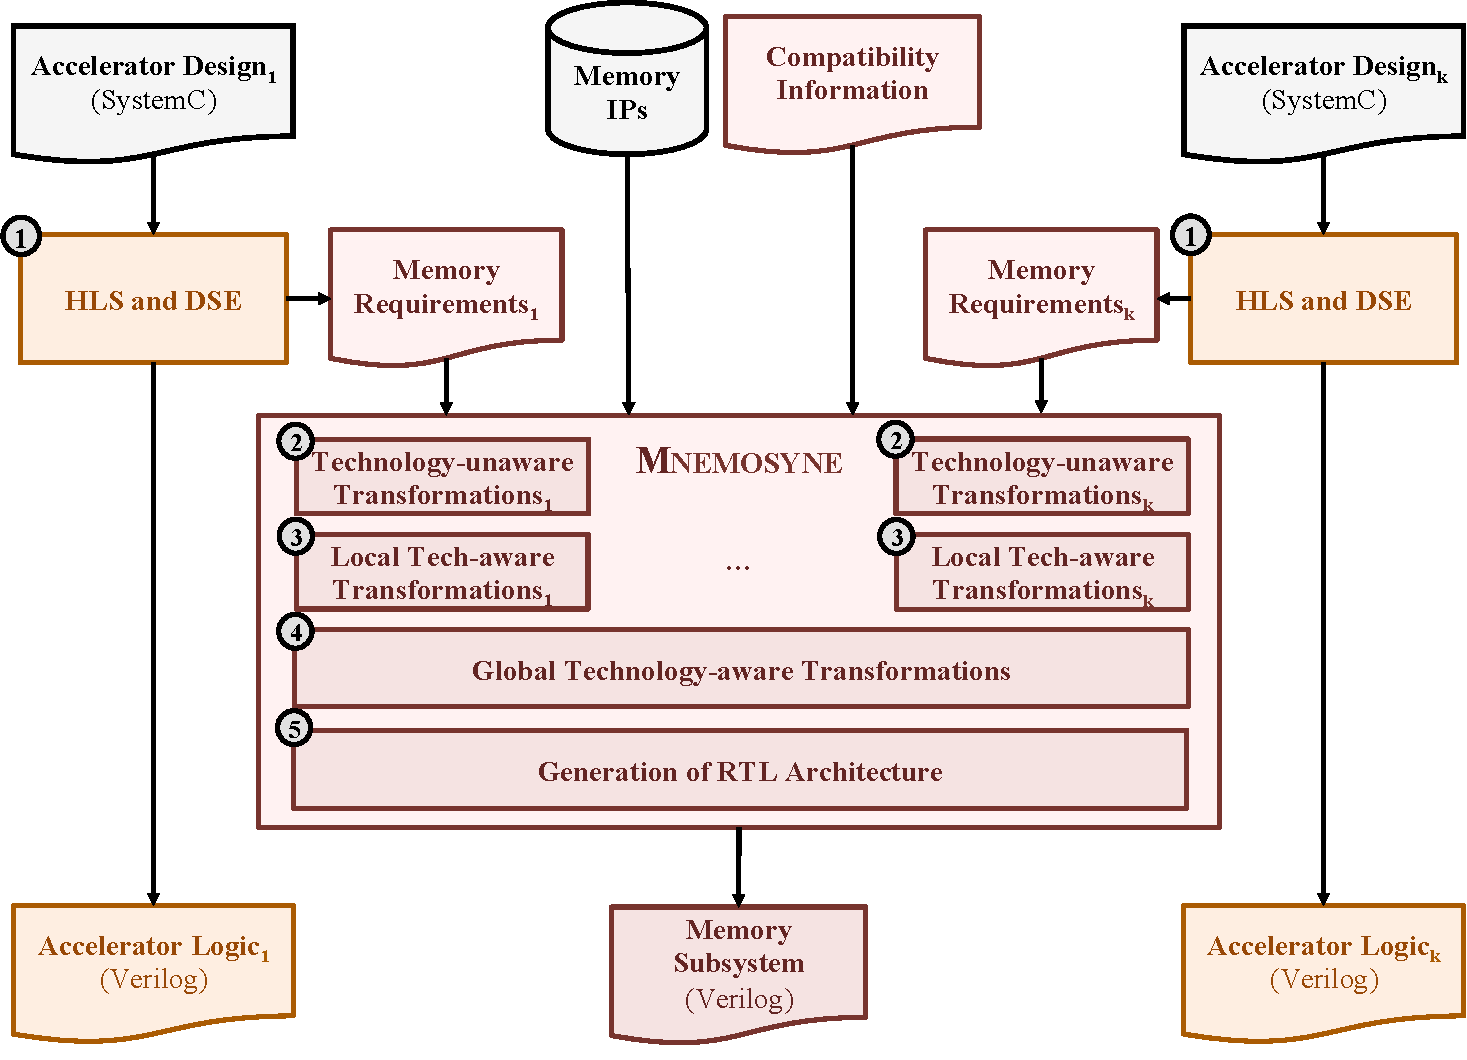
\includegraphics[height=6.4cm]{fig/methodology.pdf}
\caption{Methodology overview for accelerator memory
	design.}\label{fig:methodology}
\end{figure}

We first use a commercial HLS tool to perform design space exploration and generate
many alternative micro-architectures of each accelerator logic in order to
optimize the performance ({\it HLS and DSE}). Each implementation is
characterized by a set of data structures to be stored in the PLM and the
corresponding requirements in terms of memory interfaces ({\it Memory
Requirements$_{1\dots k}$}).
%%
We combine the information on all data structures ({\it Memory Requirements$_{1\dots k}$}),
the information on compatibilities ({\it Compatibility Information}),
and the characteristics of the memory IPs in the
{\it Memory Library} to determine an optimized architecture for each PLM. 
After selecting an implementation for each component, we determine the combined
requirements in terms of memory interfaces to access each data structure in
order to guarantee performance and functional correctness ({\it
Technology-unaware Transformations$_{1\dots k}$}).
%%
First,
we apply transformations for each accelerator ({\it Local Technology-aware
Transformations$_{1\dots k}$}). Then, we consider all accelerators at the same
time and identify when the memory IPs can be reused across different data
structures to minimize the cost of the entire memory subsystem ({\it
Global Technology-aware Transformations}). As output, we produce the RTL
description of the memory subsystem ({\it Generation of RTL Architecture}) that
can be directly integrated with the RTL descriptions of the accelerator logic
generated by the HLS tool.

\section{System-level Memory Optimization}
{\sc Mnemosyne} aims at generating an optimized memory subsystem for
one or more accelerators. The user provides information on the
data structures to be stored in the PLMs, along with additional
information on the number of memory interfaces for each accelerator
and the \textit{compatibilities} between the data structures. This
information is used to share the memory IPs across accelerators
whenever it is possible.
%
Our approach is motivated by the following observations. First, when a data
structure is not used, the associated PLM does not contain any useful data; the
corresponding memory IPs can be reused for storing another data structure, thus
reducing the total size of the memory subsystem.
%%%
Second, in some technologies, the area of a single memory IP is smaller
than the aggregated area of smaller IPs. For example, in an industrial 32nm CMOS
technology, we experimented that a 1,024$\times$32 SRAM is almost 40\%
smaller than the area of two 512$\times$32 SRAMs, due to the replicated logic
for address decoding. In these cases, it is possible to store two data
structures in the same memory IP provided that there are not conflicts on the
memory interfaces, i.e. the data structures are never accessed at the same time
with the same memory operation. Next, we formalize these situations.

To understand when two data structures can share the same memory IPs, we recall
the definition of \textit{data structure lifetime}.
\begin{quote}
{
\small
{\bf Definition.} 
The lifetime of a data structure $b$ is the interval time between the first
memory-write and the last memory-read operations to the data
structure.
\hfill $\blacksquare$
}
\end{quote}
Having two data structures with no overlapping lifetimes means that
while operating on one data structure the other remains unused.
Hence, we can use the same memory IPs to store both of them.  On the other hand,
even when two data structures have overlapping lifetimes, it is still possible
to share memory interfaces to potentially reduce the accelerator area.
\begin{quote}
{
\small
{\bf Definition.} 
Two data structures $b_i$ and $b_j$ are address-space compatible when
their lifetimes are not overlapping for the entire execution of the
accelerator. They are memory-interface compatible when it is possible
to define a \textit{total temporal ordering} of the memory operations so that
two read (resp. write) accesses to $b_i$ and $b_j$ never happen at the
same time.
\hfill $\blacksquare$
}
\end{quote}
When two data structures are memory-interface compatible, memory-read and
memory-write operations are never executed at the same time on the same data
structure.

\section{Data Allocation}

To correctly determine the number and capacity of the memory IPs for a
data structure, we must analyze the data-structure access
patterns and determine how to allocate the data.

If the read patterns can be statically analyzed and are deterministic,
it is possible to distribute the data structure across many
blocks. This technique is called \textit{cyclic partitioning} and
assigns consecutive values of the data structure to different blocks.
%%

Otherwise, it is necessary to create identical copies of the data
({\em data duplication}). This way, each memory-read interface is
assigned to a different block of data and this guarantees to access
the data without conflicts. The corresponding memory-write operations
must create consistent copies of the data in each bank.

\section{Memory Compatibility Graph}

The compatibility information provided by the designer is combined into a
\textit{Memory Compatibility Graph} (MCG), which captures the sharing
opportunities among the data structures.
\begin{quote}
{
\small
{\bf Definition.}
The Memory Compatibility Graph is a graph $MCG=(B,E)$ where each node $b
\in B$ represents a data structure to be stored in the entire memory subsystem;
an edge $e \in E$ connects two nodes when the corresponding data
structures can be assigned to the same physical memory IPs. Each edge $e \in E$
is also annotated with the corresponding type of compatibility (e.g.
address-space or memory-interface).
\hfill $\blacksquare$
}
\end{quote}
%
A MCG with no compatibility edges corresponds to implementing each
data structure in a dedicated PLM element.
%%
Increasing the number of edges into the $MCG$ corresponds to increasing the
number of compatible data structures. This can potentially increase the number
of banks that can be reused across different data structures.
An accurate compatibility graph is the key to optimize the memory subsystem of
the accelerators. In most cases, the designer has to analyze the application's
behavior or modify the interconnection topology of the accelerator to increase
sharing possibilities.
